\begin{frame}{Monte Carlo Tree Search(MCTS)}{Qu'est-ce que le MCTS}
	\begin{block}{Définition MCTS}
		Le \textbf{MCTS} :
		\begin{itemize}
			\item - Est un algorithme de \textbf{recherche arborescente}.
			\item - Utilisé pour résoudre des problèmes afin de prendre une décision.
			\item - N'utilise pas de fonction d'évaluation heuristique.
			\item - \textbf{Parcours} les possibilités \textbf{aléatoirement} avec les données précédentes.
			\item - Utilise les méthodes de \textbf{Monte Carlo} pour améliorer son efficacité.
			\item - Possède des variantes (\textbf{Coulom}, \textbf{Kocsis}, \textbf{Szepesvari}, ...).
		\end{itemize}
	\end{block}
\end{frame}

\begin{frame}{Monte Carlo Tree Search(MCTS)}{Structure}
	\begin{block}{Arbre de recherche}
		\begin{itemize}
			\item Un \textbf{arbre de recherche} est une \textbf{modélisation} des possibilités de jeu pour la simulation.
			\item Un \textbf{noeud} représente un \textbf{état} du jeu.
			\item Chaque noeud possède deux informations :
			\item\begin{itemize}
				      \item - La \textbf{valeur} de sa position.
				      \item - Le \textbf{nombre de visites} de ce noeud dans la simulation.
			      \end{itemize}
			\item Chaque feuille de cet arbre représente soit un \textbf{noeud} dont les enfants n'ont pas encore été explorés, soit un \textbf{état final} de celui-ci.
		\end{itemize}
	\end{block}
\end{frame}

\begin{frame}{Monte Carlo Tree Search(MCTS)}{Structure}
	\begin{block}{Exemple d'arbre MCTS}
		\begin{center}
			\includegraphics[width=6cm]{ressources/MCTS/tree.png}
		\end{center}
	\end{block}
\end{frame}


\begin{frame}{Monte Carlo Tree Search(MCTS)}{Structure}
	\begin{block}{Plusieurs étapes}
		\begin{itemize}
			\item 1. \textbf{Sélection}
			\item 2. \textbf{Expansion}
			\item 3. \textbf{Simulation}
			\item 4. \textbf{Rétropropagation}
			\item Répété jusqu'à la prise de décision.
		\end{itemize}
		\begin{center}
			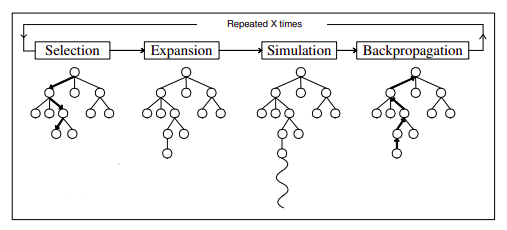
\includegraphics[width=8cm]{ressources/MCTS/MCTSEtapes}
		\end{center}
	\end{block}
\end{frame}

\begin{frame}{Monte Carlo Tree Search(MCTS)}{Sélection}
	\begin{block}{Fonctionnement de la sélection}
		\begin{columns}
			\begin{column}{7cm}
				\begin{itemize}
					\item - \textbf{Débute} à partir de la racine.
					\item \
					\item - Application \textbf{récursive} d'une \textbf{stratégie} de sélection pour \textbf{trouver} une feuille de l'arbre à étendre.
				\end{itemize}
			\end{column}
			\begin{column}{4cm}
				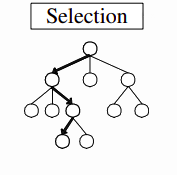
\includegraphics[width=3cm]{ressources/MCTS/Selection.png}
			\end{column}
		\end{columns}
	\end{block}
	\begin{block}{Stratégies de la sélection}
		\begin{itemize}
			\item Il existe plusieurs stratégies de sélection (\textbf{OMC}, \textbf{UCT}, \textbf{PBBM}, ...).

			\item Les \textbf{stratégies} les plus optimales font un consensus entre \textbf{exploitation} et \textbf{exploration}.
		\end{itemize}
	\end{block}
\end{frame}

\begin{frame}{Monte Carlo Tree Search(MCTS)}{Sélection}
	\begin{block}{Stratégie OMC (Objective Monte-Carlo)}
		\begin{itemize}
			\item ${U_{i}}$ une fonction d'urgence d'un mouvement avec :
			\item $U_{i} = erfc \left(\frac{v_{0} - v_{i}}{\sqrt{2}\sigma_{i}}\right)$
			\item $v_{0}$ la valeur du meilleur mouvement et $v_{j}$ la valeur du mouvement courant.
			\item $\sigma_{j}$ la déviation de $v_{j}$
			\item $erfc$ la fonction complémentaire d'erreur avec :
			\item $erfc(x) = 1 - \frac{2}{\sqrt{\pi}}\int_{x}^{\infty}e^{-u^{2}}$
			\item La probabilité $P_{m}$ pour chaque $m \in M$ avec :
			\item $P_{m} = \frac{U(m)}{\sum_{j \in S_{i}}^{}U(j)}$
			\item On choisit le prochain mouvement à simuler aléatoirement selon la probabilité $P_{m}$.
		\end{itemize}
	\end{block}
\end{frame}

\begin{frame}{Monte Carlo Tree Search(MCTS)}{Sélection}
	\begin{block}{Stratégie PBBM (Probability to be Better than Best Move)}
		\begin{itemize}
			\item Similitude avec la stratégie \textbf{OMC}.
			\item $U_{i}$ aussi une fonction d'urgence d'un mouvement avec :
			\item $U_{i} = \exp\left(-2.4\frac{v_{0} - v_{i}}{\sqrt{2(\sigma_{0}^2 + \sigma_{i}^2)}}\right) + \epsilon_{i}$
			\item $v_{0}$ la valeur du meilleur mouvement et $v_{i}$ la valeur du mouvement courant.
			\item $\sigma_{0}$ et $\sigma_{i}$ leur déviations.
			\item $\epsilon_ {i}$ une constante assurant que la fonction d'urgence ne soit pas égale à 0 avec :
			\item $\epsilon_ {i} = \frac{0.1 + 2^{-i} + a_{i}}{N}$
			\item $a_{i} = 1$ ou $0$ selon la situation.
		\end{itemize}
	\end{block}
\end{frame}

\begin{frame}{Monte Carlo Tree Search(MCTS)}{Sélection}
	\begin{block}{Stratégie UCT (Upper Confidence bounds applied to Trees)}
		\begin{itemize}
			\item La stratégie \textbf{UCT} sélectionne un noeud $k$ fils du noeud $p$ qui satisfait la formule suivante :
			      $$k \in argmax_{i\in I}\left(v_{i} + C \times \sqrt{\frac{\ln n_{p}}{n_{i}}}\right)$$
			\item $I$ un set de noeuds atteignable par le noeud $p$.
			\item $v_{i}$ la valeur du noeud $i$
			\item $n_{p}$ et $n_{p}$ le nombre de fois que les noeuds $p$ et $i$ on été visités.
			\item $C$ une constante.
		\end{itemize}
	\end{block}
\end{frame}

\begin{frame}{Monte Carlo Tree Search(MCTS)}{Sélection}
	\begin{block}{Stratégie UCB1-TUNED}
		\begin{itemize}
			\item Variante de la stratégie \textbf{UCT} qui sélectionne un noeud $k$ fils du noeud $p$ qui satisfait la formule suivante :
			      $$k \in argmax_{i\in I}\left(v_{i} + C \times \sqrt{\frac{\ln n_{p}}{n_{i}}\times \min(\frac{1}{4}, V_{i}(n_{i}))}\right)$$
			\item avec $V_{i}$ une estimation de la borne supérieur de la variance de $v_{i}$ avec comme formule :
			      $$V_{i}(n_{i}) = \left(\frac{1}{n_{i}}\sum_{t=1}^{n_{i}}R_{i,t,j}^2\right) - v_{i}^2 + \sqrt{\frac{2\ln n_{p}}{n_{i}}}$$
			\item $R_{i,t,k}$ la $t$-ième récompense obtenu au noeud $i$ pour le joueur $j$
		\end{itemize}
	\end{block}
\end{frame}

\begin{frame}{Monte Carlo Tree Search(MCTS)}{Expansion}
	\begin{block}{Fonctionnement Expansion}
		\begin{columns}
			\begin{column}{8cm}
				\begin{itemize}
					\item - \textbf{Dépend} des règles du jeu.
					\item - \textbf{Crée} un noeud à partir du noeud sélectionné si celui-ci n'est pas final.
					\item \
					\item Tout les résultats ne sont pas gardés en mémoire.
				\end{itemize}
			\end{column}
			\begin{column}{4cm}
				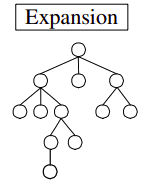
\includegraphics[width=2.5cm]{ressources/MCTS/Expansion.png}
			\end{column}
		\end{columns}
	\end{block}
	\begin{block}{Stratégies de l'expansion}
		\begin{itemize}
			\item Il existe \textbf{plusieurs stratégies} pour choisir les noeuds à garder :
			\item - \textbf{Garder seulement} un noeud par jeu simulé.
			\item - \textbf{Continuer} à \textbf{stocker} les enfants d'un noeud jusqu'à un nombre \textbf{limité} de simulations.
		\end{itemize}
	\end{block}
\end{frame}

\begin{frame}{Monte Carlo Tree Search(MCTS)}{Simulation}
	\begin{block}{Fonctionnement de la simulation}
		\begin{columns}
			\begin{column}{7cm}
				\begin{itemize}
					\item - \textbf{Réalise} une \textbf{simulation} d'une partie aléatoirement à partir du noeud étendu.
					\item \
					\item - \textbf{Continue} de \textbf{parcourir} des états de jeu jusqu'à obtenir un résultat.

				\end{itemize}
			\end{column}
			\begin{column}{3cm}
				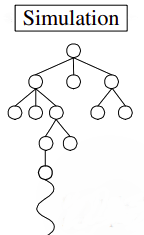
\includegraphics[width=2.2cm]{ressources/MCTS/Simulation.png}
			\end{column}
		\end{columns}
	\end{block}
	\begin{block}{Stratégies de la simulation}
		Il existe des \textbf{stratégies} de simulation qui sont difficiles à définir.

		Ces \textbf{stratégies} peuvent utiliser des \textbf{connaissances acquises} du jeu (patterns, considérations, ...)
	\end{block}
\end{frame}

\begin{frame}{Monte Carlo Tree Search(MCTS)}{Simulation}
	\begin{block}{Statégie Sequence-like Simulation}
		\begin{columns}
			\begin{column}{8cm}
				\begin{itemize}
					\item Cette stratégie est adapté au jeu de GO, et consiste à :
					\item - \textbf{Sélectionner} chaque coup à proximité du dernier coup joué $c_{0}$ avec $E$ l'ensemble des coups adjacents.
					\item - \textbf{Choisir} un coup à jouer dans $E$, en cherchant des motifs de jeu de taille 3x3 à une distance 1 de Manhattan avec $c_{0}$.
					\item - Si plusieurs motifs correspondent :
					      \textbf{choix aléatoire parmi eux}.
					\item - Si aucun est reconnu :
					      \textbf{choix aléatoire parmi tous}.
				\end{itemize}
			\end{column}
			\begin{column}{3cm}
				\vspace{1cm}
				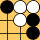
\includegraphics[width=2cm]{ressources/MCTS/3x3GridGo.png}
				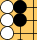
\includegraphics[width=2cm]{ressources/MCTS/3x3GridGo2.png}
			\end{column}
		\end{columns}
	\end{block}\end{frame}

\begin{frame}{Monte Carlo Tree Search(MCTS)}{Rétropropagation}
	\begin{block}{Fonctionnement de la rétropropagation}
		\begin{columns}
			\begin{column}{8cm}
				\begin{itemize}
					\item - \textbf{Propage} l'information aux \textbf{parents} du noeud récursivement avec le résultat de la simulation.
					\item - \textbf{Se propage} jusqu'au noeud le plus haut pour \textbf{diffuser} les nouvelles informations.
					\item - \textbf{Change} la valeur des noeuds visités.
					\item - \textbf{Garde} en mémoire le nombre de visites.
					\item  On pose $R_{i}$ le résultat d'une partie pour interpréter le résultat :

					      - $R_{i} = +1$ si l'IA gagne

					      - $R_{i} = -1$ si l'IA perd

					      - $R_{i} = 0$ si égalité.
				\end{itemize}
			\end{column}
			\begin{column}{4cm}
				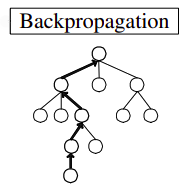
\includegraphics[width=3cm]{ressources/MCTS/Backpropagation.png}
			\end{column}
		\end{columns}
	\end{block}
\end{frame}

\begin{frame}{Monte Carlo Tree Search(MCTS)}{Stratégie Rétropropagation}
	\begin{block}{Stratégies de la rétropropagation}
		\begin{itemize}
			\item \textbf{Moyenne} : Prend la moyenne des résultats : $v_{i} = \frac{\sum_{i}^{}R_{i}}{n_{i}}$ avec $v_{i}$ la valeur du noeud et $n_i$ le nombre de fois qu'il a été visité.
			\item \textbf{Max} : Prend le max des résultats des enfants.
			\item \textbf{Moyenne informée} : Attribue de plus grandes valeurs aux meilleurs résultats.
			      On a : $v_{i} = \frac{\sum_{j}^{}(v_{j}\times n_{j}\times U_{j})}{\sum_{j}^{}(n_{j}\times U_{j})}$ avec $U_{j}$ la fonction d'urgence utilisée pour la stratégie de sélection OMC.
		\end{itemize}
	\end{block}
\end{frame}

\begin{frame}{Monte Carlo Tree Search(MCTS)}{Choix du mouvement final}
	\begin{block}{Statégies du choix du mouvement final}
		\begin{itemize}
			\item \textbf{Maximum des noeuds}: On prend le noeud qui a la plus grande valeur.
			\item \textbf{Noeud le plus robuste}: On prend le noeud qui a été visité le plus de fois.
			\item \textbf{Mix}: On prend le noeud qui est à la fois le maximum et à la fois le plus robuste.
			\item \textbf{Noeud le plus sécurisé}: On prend le noeud qui maximise une borne de confiance.
		\end{itemize}
	\end{block}
\end{frame}

\begin{frame}{Monte Carlo Tree Search(MCTS)}{Application}
	\begin{block}{Applications du MCTS}
		\begin{itemize}
			\item Le \textbf{MCTS} a été une \textbf{révolution} pour les jeux à deux joueurs.
			\item \textbf{Mogo Titan}, un programme \textbf{MCTS}, a été le premier à avoir battu un joueur professionnel de Go avec contrainte (7 pierres d'handicap).
			\item Il est utilisé par des programmes comme \textbf{MOGO}, \textbf{CRAZY STONE}, \textbf{FUEGO}, ...
			\item \textbf{AlphaGo} utilise aussi le MCTS pour sa recherche de coup.
		\end{itemize}
	\end{block}
\end{frame}